% Lightning Talk — SDSCon 2026
% Recovering Sparse Neural Connectivity from Partial Measurements
% Quilee Simeon, MIT
% 4 minutes, 8 slides
% Compile: tectonic presentation.tex  OR  pdflatex presentation.tex

\documentclass[aspectratio=169,12pt]{beamer}

% ─── Packages ───
\usepackage{graphicx}
\usepackage{amsmath,amssymb}
\usepackage{booktabs}
\usepackage{array}
\usepackage{colortbl}
\usepackage{tikz}
\usetikzlibrary{arrows.meta,positioning}

% ─── Theme: clean minimal ───
\usetheme{default}
\usecolortheme{default}
\usefonttheme{professionalfonts}
\setbeamertemplate{navigation symbols}{}
\setbeamertemplate{frametitle continuation}{}

% ─── Colors (matching poster palette) ───
\definecolor{mainblue}{HTML}{2E4057}
\definecolor{accentblue}{HTML}{0077B6}
\definecolor{accentgreen}{HTML}{2A9D8F}
\definecolor{accentred}{HTML}{E76F51}
\definecolor{lightgray}{HTML}{F5F5F5}
\definecolor{medgray}{HTML}{888888}

\setbeamercolor{frametitle}{fg=mainblue}
\setbeamercolor{title}{fg=mainblue}
\setbeamercolor{subtitle}{fg=accentblue}
\setbeamercolor{author}{fg=mainblue}
\setbeamercolor{institute}{fg=medgray}
\setbeamercolor{date}{fg=medgray}
\setbeamercolor{normal text}{fg=black,bg=white}
\setbeamercolor{itemize item}{fg=accentblue}
\setbeamercolor{itemize subitem}{fg=accentgreen}
\setbeamercolor{block title}{fg=white,bg=mainblue}
\setbeamercolor{block body}{fg=black,bg=lightgray}
\setbeamercolor{alerted text}{fg=accentred}

\setbeamerfont{frametitle}{size=\Large,series=\bfseries}
\setbeamerfont{title}{size=\large,series=\bfseries}

% ─── Frame title with blue rule ───
\setbeamertemplate{frametitle}{%
  \vspace{4pt}%
  \insertframetitle%
  \vspace{2pt}%
  {\color{accentblue}\hrule height 1.5pt}%
  \vspace{4pt}%
}

% ─── Slide numbers (subtle, bottom right) ───
\setbeamertemplate{footline}{%
  \hfill{\footnotesize\color{medgray}\insertframenumber/\inserttotalframenumber}\hspace{8pt}\vspace{4pt}%
}

% ══════════════════════════════════════════════════════════════
\begin{document}

% ──────────────────────────────────────────────────────────────
% SLIDE 1 — Title
% ──────────────────────────────────────────────────────────────
\begin{frame}[plain]
\vfill
\begin{center}
  {\Large\bfseries\color{mainblue}%
    Recovering Sparse Neural Connectivity\\[4pt]
    from Partial Measurements}\\[10pt]
  {\normalsize\color{accentblue}%
    A Covariance-Based Approach with Granger-Causality Refinement}\\[16pt]
  {\normalsize\color{mainblue} Quilee Simeon}\\[2pt]
  {\small\color{medgray} Massachusetts Institute of Technology
    \quad$\cdot$\quad \texttt{qsimeon@mit.edu}}\\[12pt]
  {\small\color{medgray} SDSCon 2026 --- Lightning Talk}
\end{center}
\vfill
\end{frame}

% ──────────────────────────────────────────────────────────────
% SLIDE 2 — Problem & Model  (0:00–0:50)
% ──────────────────────────────────────────────────────────────
\begin{frame}{Problem: Partial Observability}

\begin{columns}[T]
\begin{column}{0.52\textwidth}
  \textbf{Goal:} Recover $N{\times}N$ connectivity $W$ from
  \alert{partial measurements} across sessions.

  \vspace{3pt}
  \textbf{Dynamical model:}
  \vspace{-4pt}
  \[
    x_{t+1} = W\phi(x_t) + b_t
  \]

  \vspace{-6pt}
  Session $k$ observes $\mathcal{M}_k \subset \{1,\ldots,N\}$,
  stimulates $\mathcal{S}_k$.

  \vspace{3pt}
  \textbf{Key insight:} Pairwise covariance can be
  \textbf{accumulated across sessions} whenever $i,j$
  are co-observed.

  \vspace{2pt}
  {\small\color{medgray}\textit{C.\ elegans}, zebrafish, organoids}
\end{column}

\begin{column}{0.46\textwidth}
  \centering
  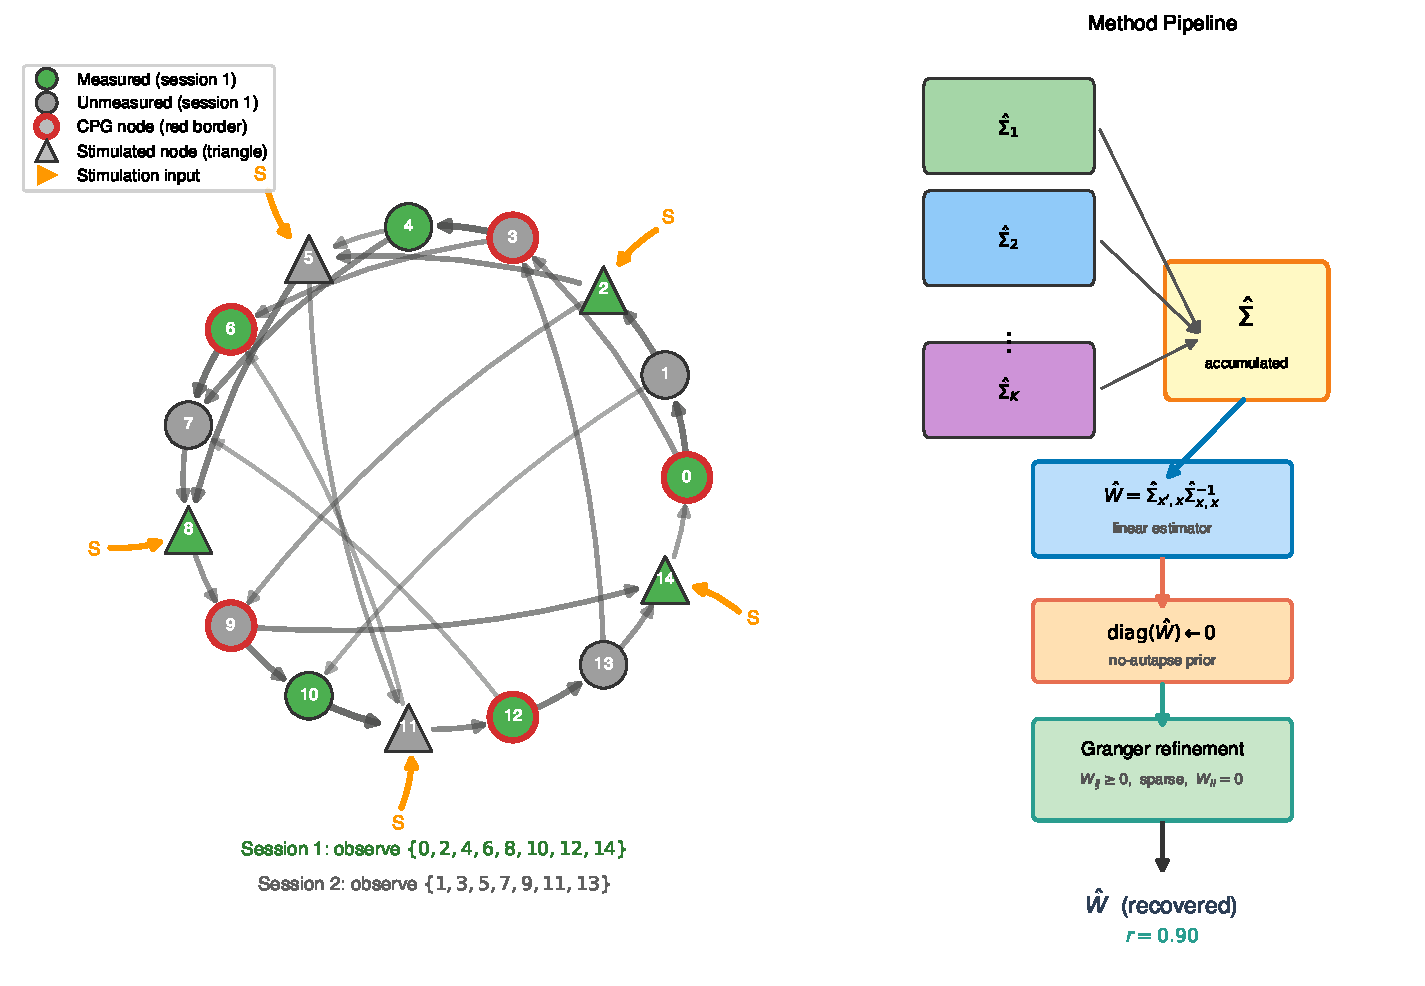
\includegraphics[width=\linewidth]{figures/fig1_problem_schematic.pdf}
\end{column}
\end{columns}

\end{frame}

% ──────────────────────────────────────────────────────────────
% SLIDE 3 — From Dynamics to Estimator  (0:50–1:30)
% ──────────────────────────────────────────────────────────────
\begin{frame}{Method: From Dynamics to Estimator}

\textbf{Step 1 --- Covariance accumulation} over $K{=}50$ sessions:
\[
  \hat{\Sigma}_{x_{t+1},x_t}(i,j) \;=\; \frac{1}{n_{ij}}
    \sum_{k:\,i,j\in\mathcal{M}_k} \hat{\Sigma}^{(k)}(i,j)
\]

\vspace{2pt}
\textbf{Step 2 --- Linear estimator.}\;
Multiply $x_{t+1}{=}W\phi(x_t){+}b_t$ by $x_t^\top$, take expectations:
\[
  \Sigma_{x_{t+1},x_t} = W\,\Sigma_{\phi(x),x} + \Sigma_{b,x}
  \quad\xrightarrow{\;\phi(x)\approx x\;}
  \quad\boxed{\;\hat{W} = \hat{\Sigma}_{x_{t+1},x_t}\;\hat{\Sigma}_{x_t,x_t}^{-1}\;}
\]
with diagonal zeroed ($W_{ii}{=}0$, no autapses) and non-negativity ($W_{ij}{\geq}0$).

\vspace{4pt}
\textbf{Step 3 --- Granger-causality refinement:} Projected gradient descent
enforcing sparsity zeros where contemporaneous covariance exceeds lagged.

\vspace{4pt}
\textbf{Identifiability:}\;
$K \geq \log(N^2/\delta)/p^2$ sessions suffice for all-pairs coverage
with probability $\geq 1{-}\delta$.

\end{frame}

% ──────────────────────────────────────────────────────────────
% SLIDE 4 — It Works  (1:20–1:45)
% ──────────────────────────────────────────────────────────────
\begin{frame}{Result: $r = 0.90$ at 66\% Coverage}

\begin{columns}[T]
\begin{column}{0.44\textwidth}
  \centering
  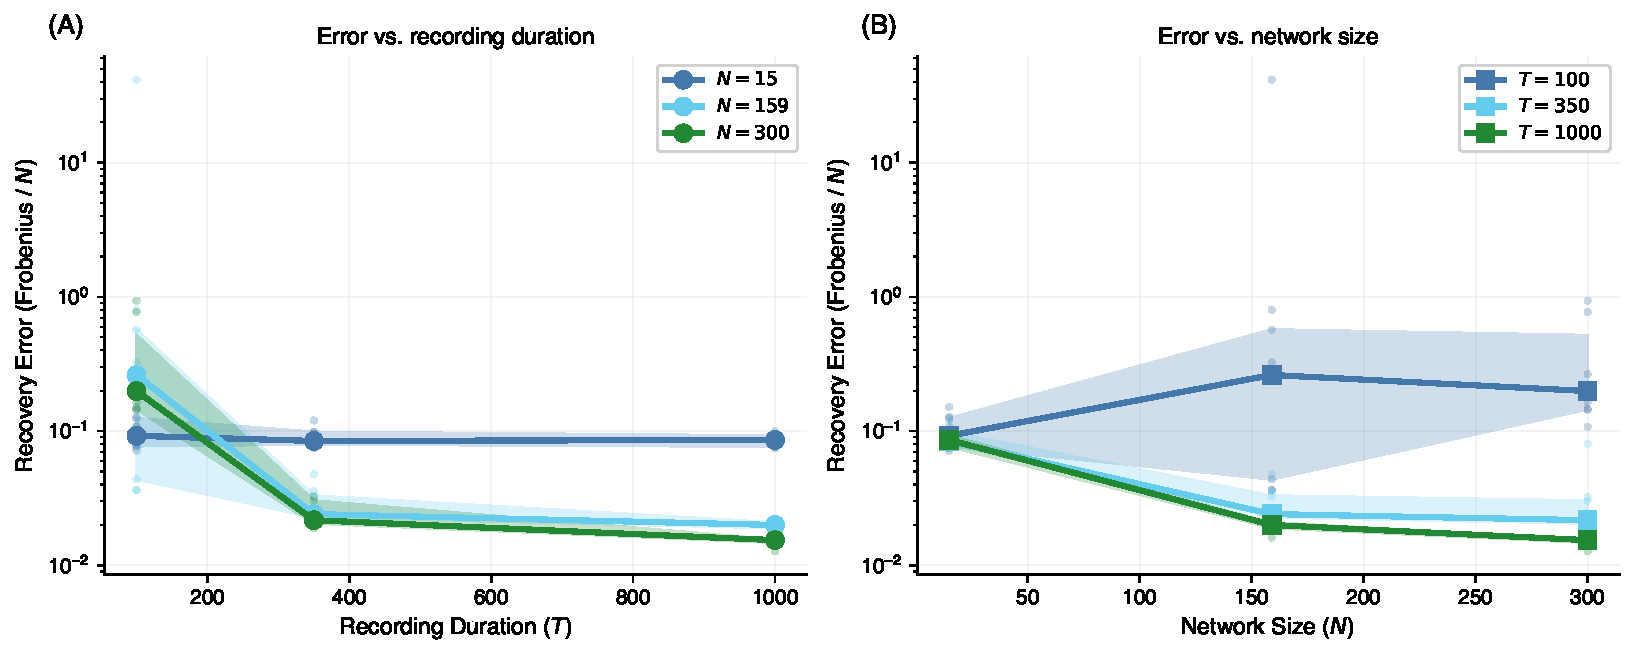
\includegraphics[width=\linewidth]{figures/fig3_scaling.pdf}

  \vspace{2pt}
  {\small Error decreases with $T$ and $N$.}
\end{column}

\begin{column}{0.50\textwidth}
  \begin{center}
  \renewcommand{\arraystretch}{1.3}
  \begin{tabular}{>{\bfseries\color{accentblue}}l l}
    Correlation & $r = 0.90$ \\
    Over same-prior & $31\%$ improvement \\
    Best error & $0.014$ ($N{=}300,T{=}1000$) \\
    Coverage & $66\%$ / session \\
    Sessions & $K{=}50$ \\
  \end{tabular}
  \end{center}

  \vspace{4pt}
  Granger refinement: precision $0.30{\to}0.40$,
  recall $0.97$ --- nearly all true edges preserved.
\end{column}
\end{columns}

\end{frame}

% ──────────────────────────────────────────────────────────────
% SLIDE 5 — Surprise: Wrong Model Wins  (1:45–2:20)
% ──────────────────────────────────────────────────────────────
\begin{frame}{Surprise: The ``Wrong'' Model Wins}

\begin{columns}[T]
\begin{column}{0.44\textwidth}
  \centering
  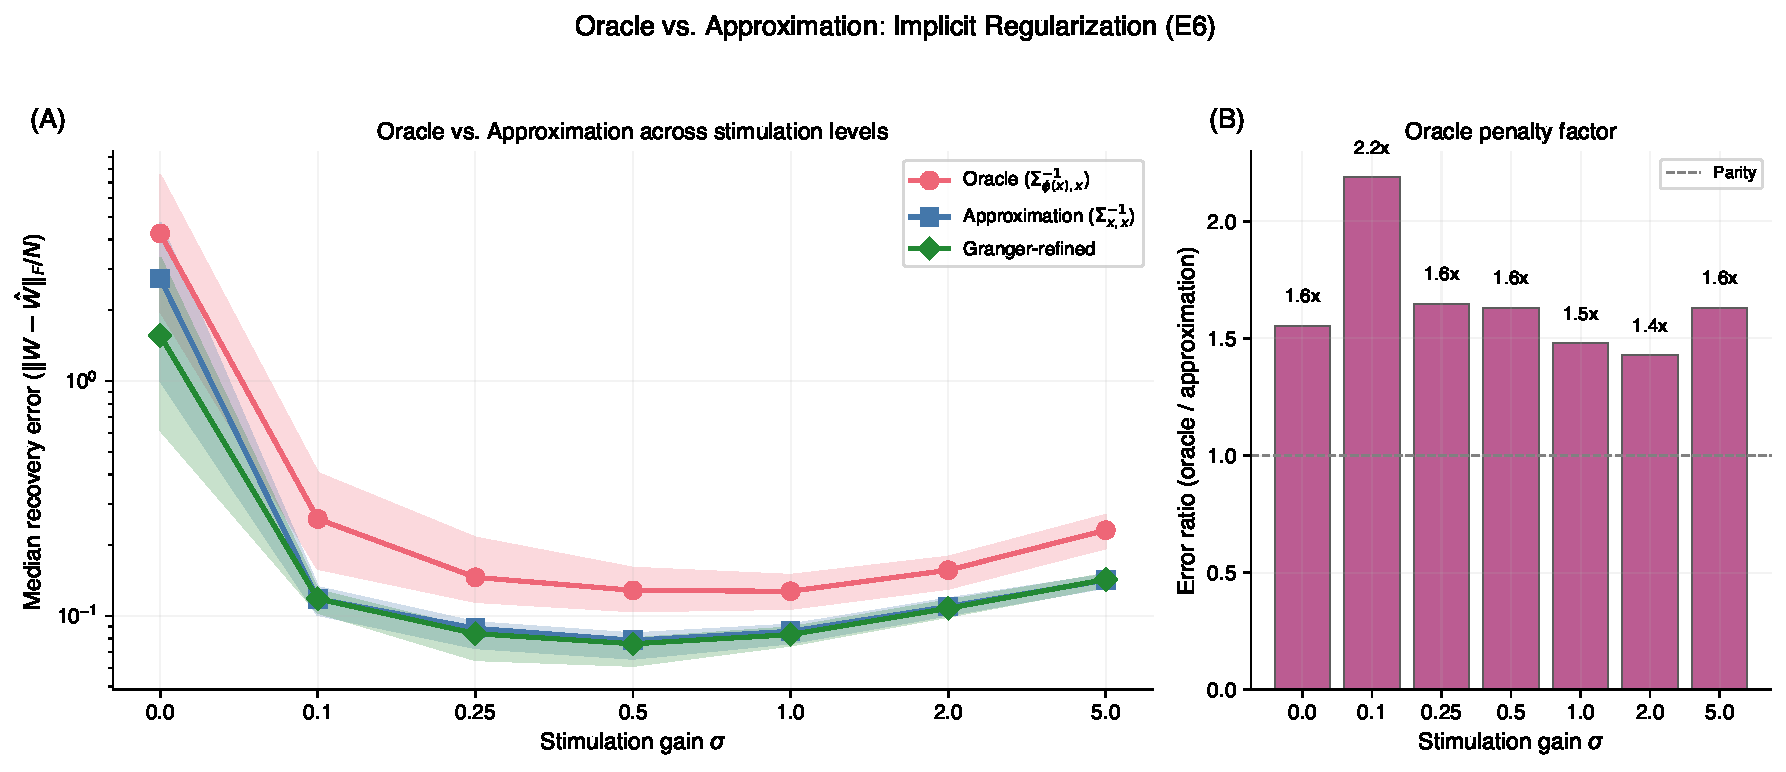
\includegraphics[width=\linewidth]{figures/fig10_oracle_comparison.pdf}

  \vspace{2pt}
  {\small Oracle with known $\phi{=}\tanh$ is
  \alert{1.5--2.7$\times$ worse}.}
\end{column}

\begin{column}{0.52\textwidth}
  We \emph{deliberately} ignore the known nonlinearity.

  \vspace{4pt}
  \textbf{Why?}\; Stein--Price identity gives
  $\Sigma_{\phi(x),x} = D\Sigma_{x,x}$
  where $D{=}\mathrm{diag}(\mathbb{E}[\mathrm{sech}^2(x_i)])$, $0{<}d_i{<}1$.

  \vspace{3pt}
  \begin{itemize}
    \item Oracle inverts $D\Sigma$ --- \alert{ill-conditioned}
    \item Linear inverts $\Sigma$ --- biased but \textbf{better-conditioned}
  \end{itemize}

  \vspace{3pt}
  {\color{accentgreen}$\Rightarrow$ \textbf{James--Stein shrinkage} in action.\\
  No need to characterize the nonlinearity.}
\end{column}
\end{columns}

\end{frame}

% ──────────────────────────────────────────────────────────────
% SLIDE 6 — Error Decomposition  (2:20–2:45)
% ──────────────────────────────────────────────────────────────
\begin{frame}{The Real Bottleneck: Intrinsic Dynamics}

The estimation error decomposes into two terms:
\[
  \underbrace{\hat{W} - W}_{\text{total}}
  \;=\;
  \underbrace{W(D - I)}_{E_1:\;\text{model mismatch}}
  \;+\;
  \underbrace{\Sigma_{b,x}\,\Sigma_{x,x}^{-1}}_{E_2:\;\text{CPG correlation}}
\]

\vspace{4pt}
\begin{center}
\renewcommand{\arraystretch}{1.3}
\begin{tabular}{lcc}
  \toprule
  \textbf{Error Source} & $\|E\|_F / N$ & \textbf{Relative} \\
  \midrule
  $E_1$: Model mismatch (linear $\approx$ tanh) & $0.080$ & $1\times$ \\
  \rowcolor{accentred!15}
  $E_2$: CPG--state correlation & $0.225$ & $\mathbf{2.8\times}$ \\
  \bottomrule
\end{tabular}
\end{center}

\vspace{6pt}
\begin{center}
  {\color{mainblue}
    Better recovery requires \textbf{modeling autonomous dynamics},\\
    not refining the nonlinear approximation.}
\end{center}

\end{frame}

% ──────────────────────────────────────────────────────────────
% SLIDE 7 — Practical Guidelines  (2:45–3:30)
% ──────────────────────────────────────────────────────────────
\begin{frame}{Practical Guidelines for Experimentalists}

\begin{columns}[T]
\begin{column}{0.54\textwidth}
  \begin{enumerate}
    \item[\color{accentgreen}\textbf{1.}]
      \textbf{Stimulate} moderately ($\sigma \approx 0.5$--$1.0$)
      on $\sim\!33\%$ of neurons

    \vspace{4pt}
    \item[\color{accentgreen}\textbf{2.}]
      \textbf{Cover} $\geq 50\%$ neurons per session

    \vspace{4pt}
    \item[\color{accentgreen}\textbf{3.}]
      \textbf{Record} $K \geq 50$ sessions with random masks

    \vspace{4pt}
    \item[\color{accentgreen}\textbf{4.}]
      \textbf{Use the linear estimator} --- simpler \emph{and} better

    \vspace{4pt}
    \item[\color{accentgreen}\textbf{5.}]
      \textbf{Next:} Model CPG dynamics (${\sim}3\times$ dominant error)
  \end{enumerate}
\end{column}

\begin{column}{0.44\textwidth}
  \centering
  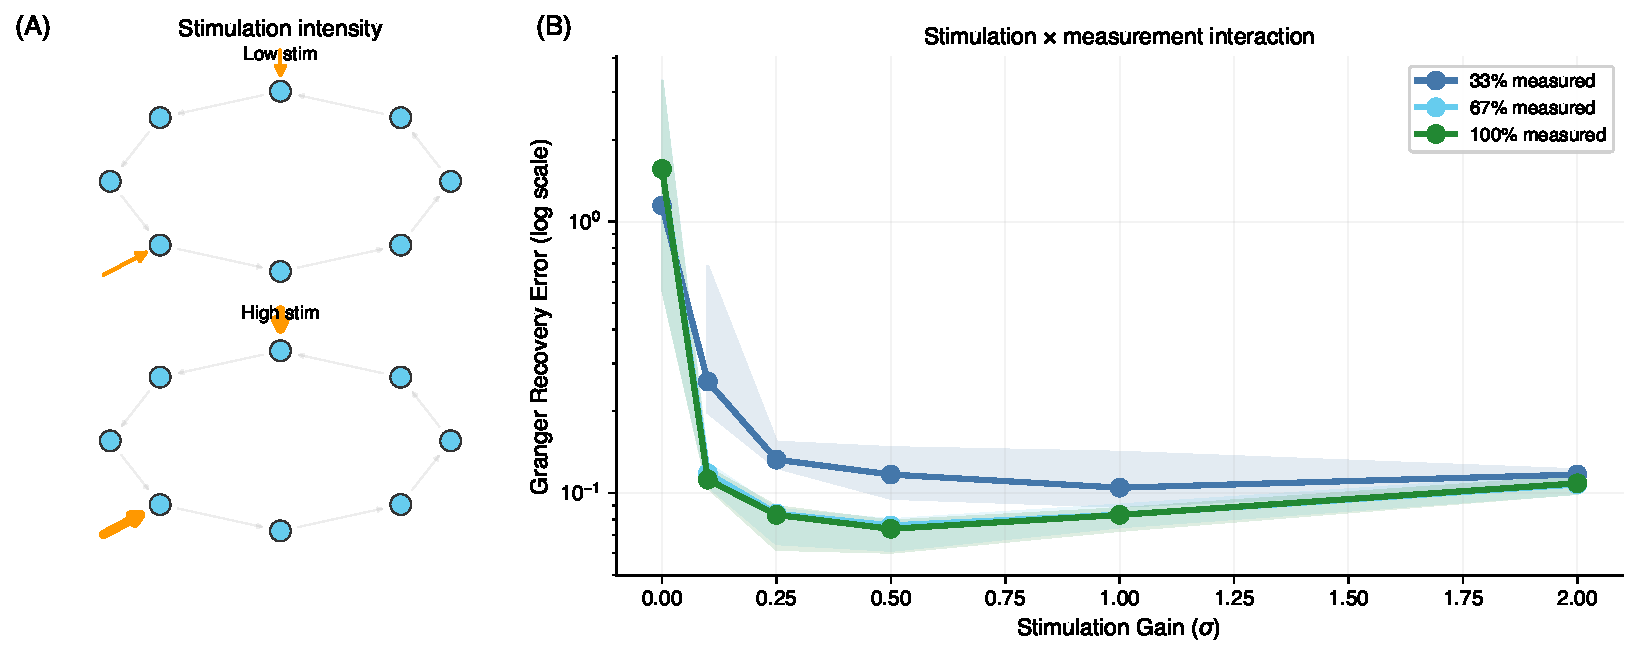
\includegraphics[width=\linewidth]{figures/fig5_stimulation.pdf}

  \vspace{6pt}
  {\small The \textbf{control--estimation tradeoff}:\\
   stimulation aids identifiability\\
   but disrupts the signal.}
\end{column}
\end{columns}

\end{frame}

% ──────────────────────────────────────────────────────────────
% SLIDE 8 — Thank You  (3:30–4:00)
% ──────────────────────────────────────────────────────────────
\begin{frame}[plain]
\vfill
\begin{center}
  {\large\color{mainblue}\bfseries
    Covariance accumulation turns partial observation\\[2pt]
    from a limitation into a feature.}

  \vspace{16pt}

  \renewcommand{\arraystretch}{1.4}
  \begin{tabular}{rl}
    {\color{accentblue}\textbf{Paper \& Code}} &
      \texttt{github.com/qsimeon/sparse\_matrix\_recovery} \\
    {\color{accentblue}\textbf{Contact}} &
      \texttt{qsimeon@mit.edu} \\
  \end{tabular}

  \vspace{16pt}
  {\LARGE\color{mainblue}\textbf{Thank you!}}\\[4pt]
  {\normalsize\color{medgray} Questions welcome at the poster session.}
\end{center}
\vfill
\end{frame}

\end{document}
